\chapter{}

We continue the study of factorization in arbitrary commutative rings. 

\begin{definition}
	Let $R$ be an integral domain. Then $R$ is \textbf{principal} (or a principal domain) if
	every ideal of $R$ is principal.  
\end{definition}

The rings $\Z$ and $\R[X]$ are both principal. 

\begin{example}
	The ring $\Z[X]$ is not principal. For example, the ideal
	$I=(2,X)$ is not principal. 
	
	First note that $I\ne\Z[X]$. In fact, if $I=\Z[X]$, then 
	$1=2f(X)+Xg(X)$ for some $f(X),g(X)\in\Z[X]$. Then
	\[
	0=\deg(1)=\deg(2f(X)+Xg(X))=\deg(f(X))+\deg(g(X))+1>0,
	\]	
	a contradiction. 
	
	If $I=(h(X))$ for some $h(X)\in\Z[X]$, then $2=h(X)g(X)$ for some $g(X)\in\Z[X]$. This
	implies that $\deg(h(X))=0$, so $h(X)=h(1)\in\Z$. In particular, $2=h(1)g(1)$ and hence
	$h(1)\in\{-1,1,2,2\}$. Since $I\ne\Z[X]$, it follows that $h(X)=h(1)\not\in\{-1,1\}$. Now      
	$X=h(X)f(X)$ for some $f(X)\in\Z[X]$. In particular, $\deg(f(X))=1$, so
	we may assume that $f(X)=a_0+a_1X$ for $a_0,a_1\in\Z$ and $a_1\ne 0$. 	
	It follows that 
	\[
	X=\pm 2f(X)=\pm2(a_0+a_1X)
	\]
	and therefore $\pm1/2=a_1\in\Z$, a contradiction.
\end{example}

\begin{example}
	Let $R=\Z[\sqrt{-5}]$.  
	The ideal $I=(2,1+\sqrt{-5})$ is not principal, so $R$ is not principal. 
	
	We first note that $I\ne R$. If not, there exist $x,y,u,v\in\Z$ such that 
	\[
	1=2(x+y\sqrt{-5})+(1+\sqrt{-5})(u+v\sqrt{-5})=(2x+u-5v)+\sqrt{-5}(2y+u+v).
	\]
	This implies that $1=2x+u-5v$ and $0=2y+u+v$. These formulas imply that
	$1=2(x+y+u-2v)$, a contradiction because $x+y+u-2v\in\Z$. 
	
	Now assume that $I=(\alpha)$. Then $\alpha\mid 2$ and $\alpha\mid 1+\sqrt{-5}$. Then
	$N(\alpha)\mid 4$ and $N(\alpha)\mid 6$, because $N(2)=4$ and $N(1+\sqrt{-5})=6$. 
	Thus $N(\alpha)\in\{1,2\}$. If we write
	$\alpha=a+b\sqrt{-5}$ for $a,b\in\Z$, then it follows that 
	$a^2+5b^2=N(\alpha)=1$ and hence $\alpha\in\mathcal{U}(R)$. 
	Therefore $I=R$, a contradiction.   
\end{example}

Sometimes primes and irreducibles coincide. 

\begin{proposition}
	Let $R$ be a principal domain and $x\in R$. 
	Then $x$ is irreducible if and only if $x$ is prime. 	
\end{proposition}

\begin{proof}
	We only need to prove that if $x$ is irreducible, then $x$ is prime. Let us
	assume that $x\mid yz$. Let $I=(x,y)$. Since $R$ is principal, $I=(a)$ for some $a\in R$. In particular, $x=ab$ for some $b\in R$. Since $x$ is irreducible, $a\in\mathcal{U}(R)$ or
	$b\in\mathcal{U}(R)$. If $a\in\mathcal{U}(R)$, then $I=R$ and hence 
	$1=xr+ys$ for some $r,s\in R$. Thus
	\[
	z=z1=z(xr+ys)=zxr+zys
	\]
	and therefore $x\mid z$. If $b\in\mathcal{U}(R)$, then $x$ and $a$ are associate, 
	in $R$. Thus $I=(x)=(a)$ and hence $xt=y$ for some $t\in R$, that is $x\mid y$.  
\end{proof}

In the integers primes and irreducible coincide. This happens 
because $\Z$ is a principal domain.

\begin{example}
	Since $\Z[\sqrt{-3}]$ have irreducible elements that are not prime, it follows that
	$\Z[\sqrt{-3}]$ is not a principal domain.
\end{example}

\begin{definition}
	Let $R$ be an integral domain. We say that $R$ is an \textbf{euclidean domain}
	if there exists a map $\varphi\colon R\setminus\{0\}\to\Z_{\geq0}$ such that
	for every $x,y\in R$ with $y\ne 0$ there exist $q,r\in R$ such that 
	$x=qy+r$, where $r=0$ or $\varphi(r)<\varphi(y)$. 
\end{definition}

Note that in the definition of euclidean domains we do not ask for the uniqueness 
of the quotient and the remainder. In fact, 
we will meet important examples of euclidean domains where uniqueness
in the division algorithm is not achieved. 

\begin{example}
	$\Z$ is an euclidean domain with $\varphi(x)=|x|$.
\end{example}

Do we have uniqueness in the previous example? 	

\begin{example}
	$\R[X]$ is an euclidean domain with $\varphi(f(X))=\deg(f(X))$. 	
\end{example}

The previous examples shows why in the definition of an euclidean domain 
we consider $\varphi\colon R\setminus\{0\}\to\Z_{\geq0}$. 

\begin{example}
	Let $R=\Z[i]$. Then $R$ is an euclidean domain with $\varphi(\alpha)=N(\alpha)$. Let 
	$\alpha=a+ib$ and $\beta=c+id\ne 0$. Then
	\[
	\frac{\alpha}{\beta}=\frac{a+ib}{c+id}=r+is
	\]
	for some $r,s\in\Z$. Let $m,n\in\Z$ be such that $|r-m|\leq 1/2$ and 
	$|s-n|\leq 1/2$. If $\delta=m+in$ and $\gamma=\alpha-\beta\delta$, then 
	$\gamma\in R$, $\delta\in R$ and $\alpha=\beta\delta+\gamma$. If $\gamma\ne0$, then
	\begin{align*}
	\varphi(\gamma)&=\varphi\left(\beta\left(\frac{\alpha}{\beta}-\delta\right)\right)
	=\varphi(\beta)\varphi\left(\frac{\alpha}{\beta}-\delta\right)\\
	&=\varphi(\beta)\varphi((r-m)+i(s-n))
	=\varphi(\beta)((r-m)^2+(s-n)^2)\\
	&\leq\varphi(\beta)(1/4+1/4)\\
	&<\varphi(\beta).
	\end{align*}	
\end{example}

In $\Z[i]$ the division algorithm does not have uniqueness. In fact, 
if $\alpha,\beta\in\Z[i]$ and $\alpha=\beta\delta+\gamma$ 
for some $\delta,\gamma\in\Z[i]$, 
then there are up to four possibilities 
for the remainder $\gamma$.


\begin{example}
	Let $R=\Z[i]$ and 
	$\alpha=-1+i$ and $\beta=1+2i$. Let $I=(\beta)$ be the ideal of $R$ generated by $\beta$. 
	First note that
	\[
	I=(\beta)=(1+2i)R=(1+2i)\Z+(1+2i)\Z i=(1+2i)\Z+(-2+i)\Z.
	\]  
	This allows us to draw the lattice of elements of $I$, 
	that is the lattice formed by the multiples of $\beta$, see Figure~\ref{fig:Z[i]}. 
	Since $\alpha-\gamma\in I=(\beta)$, there are at most four possibilites for writing
	the division algorithm. 
	In our particular example, we find three possible cases:
	\begin{enumerate}
		\item If $\alpha-\gamma=\beta_0$, where $0=\beta_0=\beta 0$, 
			then $\gamma=\alpha=-1+i$ and 
				\[
				-1+i=(1+2i)0+(-1+i)
				\]
				with $N(-1+i)=2<N(\beta)=5$. 
		\item If $\alpha-\gamma=\beta_1$, where $-2+i=\beta_1=\beta i$, then 
			$\gamma=-1$ and 
			\[
			-1+i=(1+2i)i+(-1)
			\]
			with $N(-1)=1<N(\beta)=5$. 
		\item If $\alpha-\gamma=\beta_2$, where $-1+3=\beta_2i=\beta (1+i)$, 
			then $\gamma=2i$ and  
			\[
			-1+i=(1+2i)(1+i)+(-2i)
			\]
			and $N(-2i)=4<N(\beta)=5$. 
	\end{enumerate}
%	We note that the case $\alpha-\gamma=\beta$ yields $\gamma=-2-i$ and thus
%	$N(\gamma)=N(\beta)=5$.  
\end{example}

\begin{figure}
	\centering
%	\begin{tikzcd}
%	\bullet & \beta_2 & \bullet & \bullet \\
%	\bullet & \bullet & \bullet & \beta \\
%	{\beta_1} & \alpha & i & \bullet \\
%	\bullet & -1 & {\beta_0} & 1
%	\arrow[dashed, no head, from=3-2, to=3-3]
%	\arrow[dashed, no head, from=3-3, to=2-3]
%	\arrow[dashed, no head, from=2-3, to=2-2]
%	\arrow[dashed, no head, from=2-2, to=3-2]
%	\arrow[dashed, no head, from=3-2, to=3-1]
%	\arrow[dashed, no head, from=3-1, to=2-1]
%	\arrow[dashed, no head, from=2-2, to=2-1]
%	\arrow[dashed, no head, from=1-1, to=2-1]
%	\arrow[dashed, no head, from=1-1, to=1-2]
%	\arrow[dashed, no head, from=1-2, to=2-2]
%	\arrow[dashed, no head, from=1-2, to=1-3]
%	\arrow[dashed, no head, from=1-3, to=2-3]
%	\arrow[no head, from=3-1, to=1-2]
%	\arrow[dashed, no head, from=1-3, to=1-4]
%	\arrow[dashed, no head, from=1-4, to=2-4]
%	\arrow[dashed, no head, from=2-3, to=2-4]
%	\arrow[dashed, no head, from=3-3, to=3-4]
%	\arrow[dashed, no head, from=3-4, to=2-4]
%	\arrow[no head, from=1-2, to=2-4]
%	\arrow[no head, from=3-1, to=4-3]
%	\arrow[no head, from=4-3, to=2-4]
%	\arrow[dashed, no head, from=3-1, to=4-1]
%	\arrow[dashed, no head, from=3-2, to=4-2]
%	\arrow[dashed, no head, from=3-3, to=4-3]
%	\arrow[dashed, no head, from=3-4, to=4-4]
%	\arrow[dashed, no head, from=4-4, to=4-3]
%	\arrow[dashed, no head, from=4-3, to=4-2]
%	\arrow[dashed, no head, from=4-2, to=4-1]
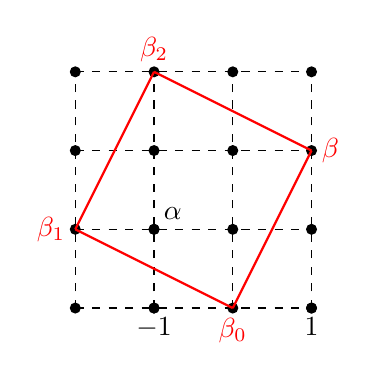
\begin{tikzpicture} 
\draw[dashed] (0,0) grid (3,3); 
\foreach \i in {0,...,3}     
\foreach \j in {0,...,3}         
\fill (\i,\j) circle (2pt);  
\draw[red,thick] 
(2,0)--(0,1) node[anchor=east] {$\beta_1$} 
(0,1)--(1,3) node[anchor=south] {$\beta_2$} 
(1,3)--(3,2) node[anchor=west] {$\beta$} 
(3,2)--(2,0) node[anchor=north] {$\beta_0$} ;
\fill (1,1) circle (2pt) node[anchor=south west] {$\alpha$}  ;
\fill (1,0) circle (2pt) node[anchor=north] {$-1$}  ;
\fill (3,0) circle (2pt) node[anchor=north] {$1$}  ;
\end{tikzpicture}
\caption{Division algorithm in $\Z[i]$.}
\label{fig:Z[i]}
\end{figure}

We know that $\Z$ and $\R[X]$ are both principal. The proofs 
are very similar, as both use the division algorithm essentially in the same way. 
The following result takes advantage of this fact. 

\begin{proposition}
	Let $R$ be an euclidean domain. Then $R$ is principal.	
\end{proposition}

\begin{proof}
	Let $I$ be an ideal of $R$. If $I=\{0\}$, then $I=(0)$ and hence 
	it is principal. So we may
	assume that $I\ne\{0\}$. Let $y\in I\setminus\{0\}$ be such that
	$\varphi(y)$ is minimal. We claim that $I=(y)$. 
	If $z\in I$, then $z=yq+r$, where $r=0$ or $\varphi(r)<\varphi(y)$. 
	The minimality of $\varphi(y)$ implies that $r=0$. Thus $z=yq\in (y)$ and 
	it follows that 
	$I=(y)$. 
\end{proof}

\begin{example}\
	Since $\Z[i]$ is euclidean, then it is principal.
\end{example}
 
\begin{example}
	The rings $\Z[\sqrt{-5}]$ and $\Z\left[\sqrt{-3}\right]$ are
	not principal. Why?
\end{example}

The ring $\Z[\frac{1+\sqrt{-19}}{2}]$ is an 
example of a ring that is principal and not euclidean. We will not prove this
fact in these notes. For a proof see...

\begin{definition}
	Let $R$ be an integral domain. Then $R$ is a 
	\textbf{unique factorization domain}
	if the following statements hold:
	\begin{enumerate}
	\item Each $x\in R\setminus\{0\}$ that is not a unit can be written as $x=c_1\cdots c_n$ for irreducibles $c_1,\dots,c_n$. 
	\item If $x=c_1\cdots c_n=d_1\cdots d_m$ for irreducibles $c_1,\dots,c_n$ and $d_1,\dots,d_m$, then $n=m$ and there exists $\sigma\in\Sym_n$ such that $c_i$ and $d_{\sigma(i)}$ are
		associate for all $i\in\{1,\dots,n\}$. 
	\end{enumerate}
\end{definition}

It is important to remark that some rings 
have factorizations and this factorization is not unique. 
In fact, if $N$ is a square-free integer, $\Z[\sqrt{N}]$ is noetherian and hence it has  
has factorization. This fact will be proved in the proof of the following theorem. 
However, not all these rings with be euclidean domains. 

\begin{theorem}
	Let $R$ be a principal domain. 
	Then $R$ is a unique factorization domain.
\end{theorem}

\begin{proof}
	We divide the proof into three steps. 
	\begin{claim}
		$R$ is noetherian. 	
	\end{claim}
	
	Let $I_1\subsetneq I_2\subsetneq$ be a sequence of ideals of $R$.  
	Since $R$ is principal, each $I_j$ is principal, 
	say $I_j=(a_j)$ for some $a_j\in R$, so the sequence is of the form
	$(a_1)\subsetneq (a_2)\subsetneq\cdots$. Since $I=\cup_{i\geq1}(a_i)$ is an ideal of $R$, 
	there exists $x\in R$ such that $I=(x)$. Since $x\in (a_n)$ for some $n\in\Z_{>0}$, 
	it follows that $(a_k)\subseteq I=(x)\subseteq (a_n)$ for all $k\in\Z_{>0}$. 
	
	\begin{claim}
		$R$ admits factorizations. 	
	\end{claim}
	
	Let $x\in R\setminus\{0\}$ be such that $x\not\in\mathcal{U}(R)$. If $x$ is irreducible, 
	there is nothing to prove. If not, $x=x_1x_2$ with $x_1\not\in\mathcal{U}(R)$ and
	$x_2\not\in\mathcal{U}(R)$. If $x_1$ and $x_2$ are both irreducibles, 
	we are done. If not, say $x_1$ can be written as $x_1=x_{11}x_{12}$ with
	$x_{11}\not\in\mathcal{U}(R)$ and $x_{12}\not\in\mathcal{U}(R)$. If this process
	does not terminate, it means that there is a sequence of ideals
	\[
	(x)\subsetneq (x_1)\subsetneq (x_{11})\subsetneq\cdots 
	\]
	that does not stabilize, which contradicts the fact that $R$ is noetherian.  
	
	\begin{claim}
		$R$ admits unique factorization.	
	\end{claim}
	
	Let $x\in R$ be such that $x$ factorizes into irreducibles as 
	$x=c_1\cdots c_n=d_1\cdots d_m$. We may assume that $n\leq m$. We proceed by 
	induction on $m$. If $m=1$, then 
	$n=1$ and $c_1=d_1$. If $m>1$, then, since $c_1$ is prime and 
	$c_1\mid d_1\cdots d_m$, it follows that $c_1\mid d_j$ for some $j$, say $c_1\mid d_1$ (here is precisely where the permutation $\sigma$ appears). Since
	$d_1$ is irreducible, $c_1$ and $d_1$ are associate, that is
	$c_1=ud_1$ for some $u\in\mathcal{U}(R)$. Then
	\[
	c_1c_2\cdots c_n=(ud_1)c_2\cdots c_n=d_1d_2\cdots d_m. 
	\]
	Since $d_1\ne 0$,  
	\[
	d_1(uc_2\cdots c_n-d_2\cdots d_m)=0,
	\]
	which implies that $(uc_2)\cdots c_n=d_2\cdots d_m$ because $R$ is an integral domain. Note
	that $uc_2$ is irreducible and hence 
	the claim follows by the inductive hypothesis. 
\end{proof}

It is interesting to remark that the proof 
of the previous theorem is exactly the proof
one does for $\Z$. 

\begin{example}
	The ring $\Z[i]$ is a unique factorization domain. 	
\end{example}

\begin{example}
	The ring $R=\Z[\sqrt{-6}]$ is not a unique factorization domain. In fact,
	\[
	10=2\cdot 5=(2+\sqrt{-6})(2-\sqrt{-6}).
	\]	
	Note that $N(a+b\sqrt{-6})=a^2+6b^2\ne 2$. This implies that $2$ is irreducible, as 
	if $2=\alpha\beta$, then $4=N(2)=N(\alpha)N(\beta)$. 
	Similarly, $5$ is irreducible. It is an exercise to prove that 
	$2+\sqrt{-6}$ and $2-\sqrt{-6}$ are both irreducible. 
\end{example}
